\documentclass[%
%10pt,
%varwidth=false,
%crop=true,
border={0mm 0mm 0mm 0mm}]{standalone}
\usepackage[T1]{fontenc}
\usepackage[utf8]{inputenc}
\usepackage[auto]{microtype}
%\usepackage{cmbright}
\usepackage{arev}
\usepackage{amsmath, amssymb, amsfonts, icomma}
\usepackage[version=4]{mhchem}
\usepackage{tikz}
\usetikzlibrary{positioning}
\usepackage{chemplants-tub}
\usepackage{xcolor}
%define stream tip, default is stealth
\setchpstreamtip{latex}
\setchpmainstreamthickness{thick}
%\setchpunitthickness{very thick}

\pgfdeclarelayer{bg}    % declare background layer
\pgfsetlayers{bg,main}  % set the order of the layers (main is the standard layer)

\definecolor{signalgruen}{RGB}{49,127,67}    % RAL 6032 Wasser
\definecolor{signalrot}{RGB}{155,36,35}      % RAL 3001 Dampf
\definecolor{signalgrau}{RGB}{150,153,146}   % RAL 7004 Luft
\definecolor{signalgelb}{RGB}{229,190,001}   % RAL 1003 brennbare und nicht brennbare Gase
\definecolor{signalorange}{RGB}{208,93,40}   % RAL 2010 Säuren
\definecolor{signalviolett}{RGB}{132,76,130} % RAL 4008 Laugen
\definecolor{signalbraun}{RGB}{121,77,62}    % RAL 8002 brennbare und nicht brennbare Flüssigkeiten
\definecolor{signalblau}{RGB}{30,45,110}     % RAL 5005 Sauerstoff

% TABLEAU-10
\definecolor{Tab10-A}{RGB}{78, 121, 167}
\definecolor{Tab10-B}{RGB}{242, 142, 43}
\definecolor{Tab10-C}{RGB}{225, 87, 89}
\definecolor{Tab10-D}{RGB}{118, 183, 178}
\definecolor{Tab10-E}{RGB}{89, 161, 79}
\definecolor{Tab10-F}{RGB}{237, 201, 72}
\definecolor{Tab10-G}{RGB}{176, 122, 161}
\definecolor{Tab10-H}{RGB}{255, 157, 167}
\definecolor{Tab10-I}{RGB}{156, 117, 95}
\definecolor{Tab10-J}{RGB}{186, 176, 172}

\begin{document}
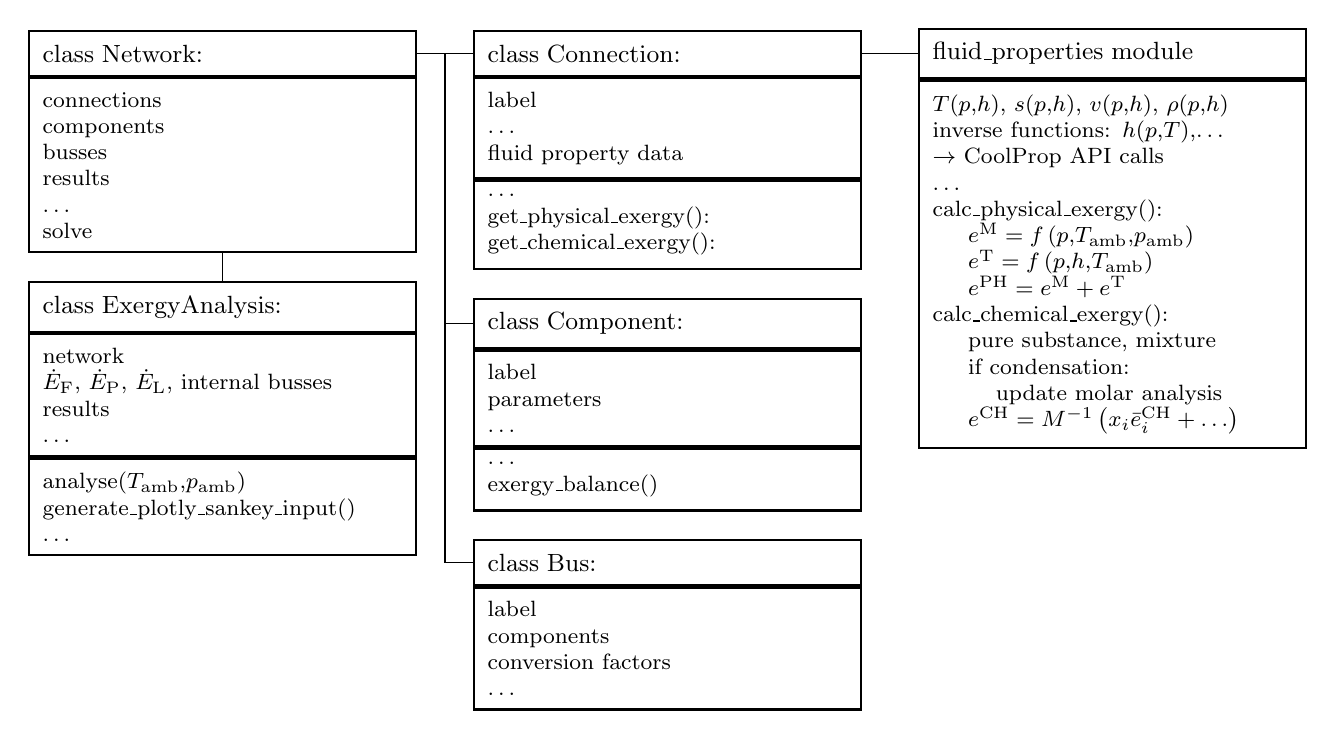
\begin{tikzpicture}[font=\footnotesize] 
%

%help grid and labels
%\draw[help lines] (-2,-3) grid (15,5);
%\foreach \pos in {-2,-1,0,1,2,3,4,5,6,7,8,9,10,11,12,13,14,15}
%\draw[shift={(\pos,-3)}] (0pt,2pt) -- (0pt,-2pt) node[below] {$\pos$};
%\foreach \pos in {-3,-2,-1,0,1,2,3,4,5}
%\draw[shift={(-2,\pos)}] (2pt,0pt) -- (-2pt,0pt) node[left] {$\pos$};

%%% nodes and boxes

%%% NETWORK
\node [rectangle, draw=black, minimum width=140pt, text width= 130pt, thick, inner sep=5pt, align=left] (network-cl) at (1,4) {\small class Network:};
\node [rectangle, draw=black, minimum width=140pt, text width= 130pt, thick, inner sep=5pt, align=left, anchor=north] (network-sub) at (network-cl.south) {connections\\ components\\ busses\\ results\\ \ldots \\ solve};

%%% EXERGY ANALYSIS
\node [rectangle, draw=black, minimum width=140pt, text width= 130pt, thick, inner sep=5pt, align=left, below = 10pt of network-sub] (exergy-cl) {\small class ExergyAnalysis:};
\node [rectangle, draw=black, minimum width=140pt, text width= 130pt, thick, inner sep=5pt, align=left, anchor=north] (exergy-sub1) at (exergy-cl.south) {network\\ $\dot E_\text{F}$, $\dot E_\text{P}$, $\dot E_\text{L}$, internal busses\\ results\\ \ldots};
\node [rectangle, draw=black, minimum width=140pt, text width= 130pt, thick, inner sep=5pt, align=left, anchor=north] (exergy-sub2) at (exergy-sub1.south) {analyse$(T_\text{amb},p_\text{amb})$\\ generate\_plotly\_sankey\_input()\\ \ldots};

%%% CONNECTION
\node [rectangle, draw=black, minimum width=140pt, text width= 130pt, thick, inner sep=5pt, align=left, right = 20pt of network-cl] (connection-cl) {\small class Connection:};
\node [rectangle, draw=black, minimum width=140pt, text width= 130pt, thick, inner sep=5pt, align=left, anchor=north] (connection-sub1) at (connection-cl.south) {label\\ \ldots \\fluid property data};
\node [rectangle, draw=black, minimum width=140pt, text width= 130pt, thick, inner sep=5pt, align=left, anchor=north] (connection-sub2) at (connection-sub1.south) {\ldots \\get\_physical\_exergy():\\ get\_chemical\_exergy():};

%%% COMPONENT
\node [rectangle, draw=black, minimum width=140pt, text width= 130pt, thick, inner sep=5pt, align=left, below = 10pt of connection-sub2] (component-cl) {\small class Component:};
\node [rectangle, draw=black, minimum width=140pt, text width= 130pt, thick, inner sep=5pt, align=left, anchor=north] (component-sub1) at (component-cl.south) {label\\ parameters\\ \ldots};
\node [rectangle, draw=black, minimum width=140pt, text width= 130pt, thick, inner sep=5pt, align=left, anchor=north] (component-sub2) at (component-sub1.south) {\ldots \\ exergy\_balance()};

%%% BUS
\node [rectangle, draw=black, minimum width=140pt, text width= 130pt, thick, inner sep=5pt, align=left, below = 10pt of component-sub2] (bus-cl) {\small class Bus:};
\node [rectangle, draw=black, minimum width=140pt, text width= 130pt, thick, inner sep=5pt, align=left, anchor=north] (bus-sub) at (bus-cl.south) {label\\ components\\ conversion factors\\ \ldots};

%%% FLUID PROPERTIES
\node [rectangle, draw=black, minimum width=140pt, text width= 130pt, thick, inner sep=5pt, align=left, right = 20pt of connection-cl] (fluids-mod) {\small fluid\_properties module};
\node [rectangle, draw=black, minimum width=140pt, text width= 130pt, thick, inner sep=5pt, align=left, anchor=north] (fluids-sub) at (fluids-mod.south) {$T(p,h)$, $s(p,h)$, $v(p,h)$, $\rho(p,h)$\\ inverse functions: $h(p,T)$,\ldots \\ $\rightarrow$ CoolProp API calls \\ \ldots \\ calc\_physical\_exergy(): \\ \hspace{10pt} $e^\text{M}=f\left(p,T_\text{amb},p_\text{amb}\right)$\\ \hspace{10pt} $e^\text{T}=f\left(p,h,T_\text{amb}\right)$\\ \hspace{10pt} $e^\text{PH}=e^\text{M}+e^\text{T}$\\ calc\_chemical\_exergy():\\ \hspace{10pt} pure substance, mixture\\ \hspace{10pt} if condensation:\\ \hspace{20pt} update molar analysis\\ \hspace{10pt} $e^\text{CH}=M^{-1}\left(x_i \bar{e}_i^\text{CH} + \ldots\right)$};


%%% connections, arrows

\draw [solid] (network-sub) -- (exergy-cl);
\draw [solid] (network-cl) -- (connection-cl);
\draw [solid] (network-cl.east) -- ++(10pt,0) |- (component-cl.west);
\draw [solid] (network-cl.east) -- ++(10pt,0) |- (bus-cl.west);
\draw [solid] (connection-cl) -- (fluids-mod);

\end{tikzpicture}

\end{document}